\chapter{Was ist ein Compiler}
In der Informatik beschreibt Compiler ein Programm, das Code aus einer Programmiersprache in eine andere übersetzt. In dieser Hinsicht gleichen Compiler Übersetzern für Menschensprache.
Jedoch unterscheidet sich ein Compiler grundsätzlich von Übersetzern in der Erwartungshaltung, die an sie gestellt wird. Menschensprache ist sehr komplex und [...]
\newline
\newline
Ein Compiler ist traditionell nach folgendem Schema aufgebaut.

\begin{figure}[h!]
    \centering
    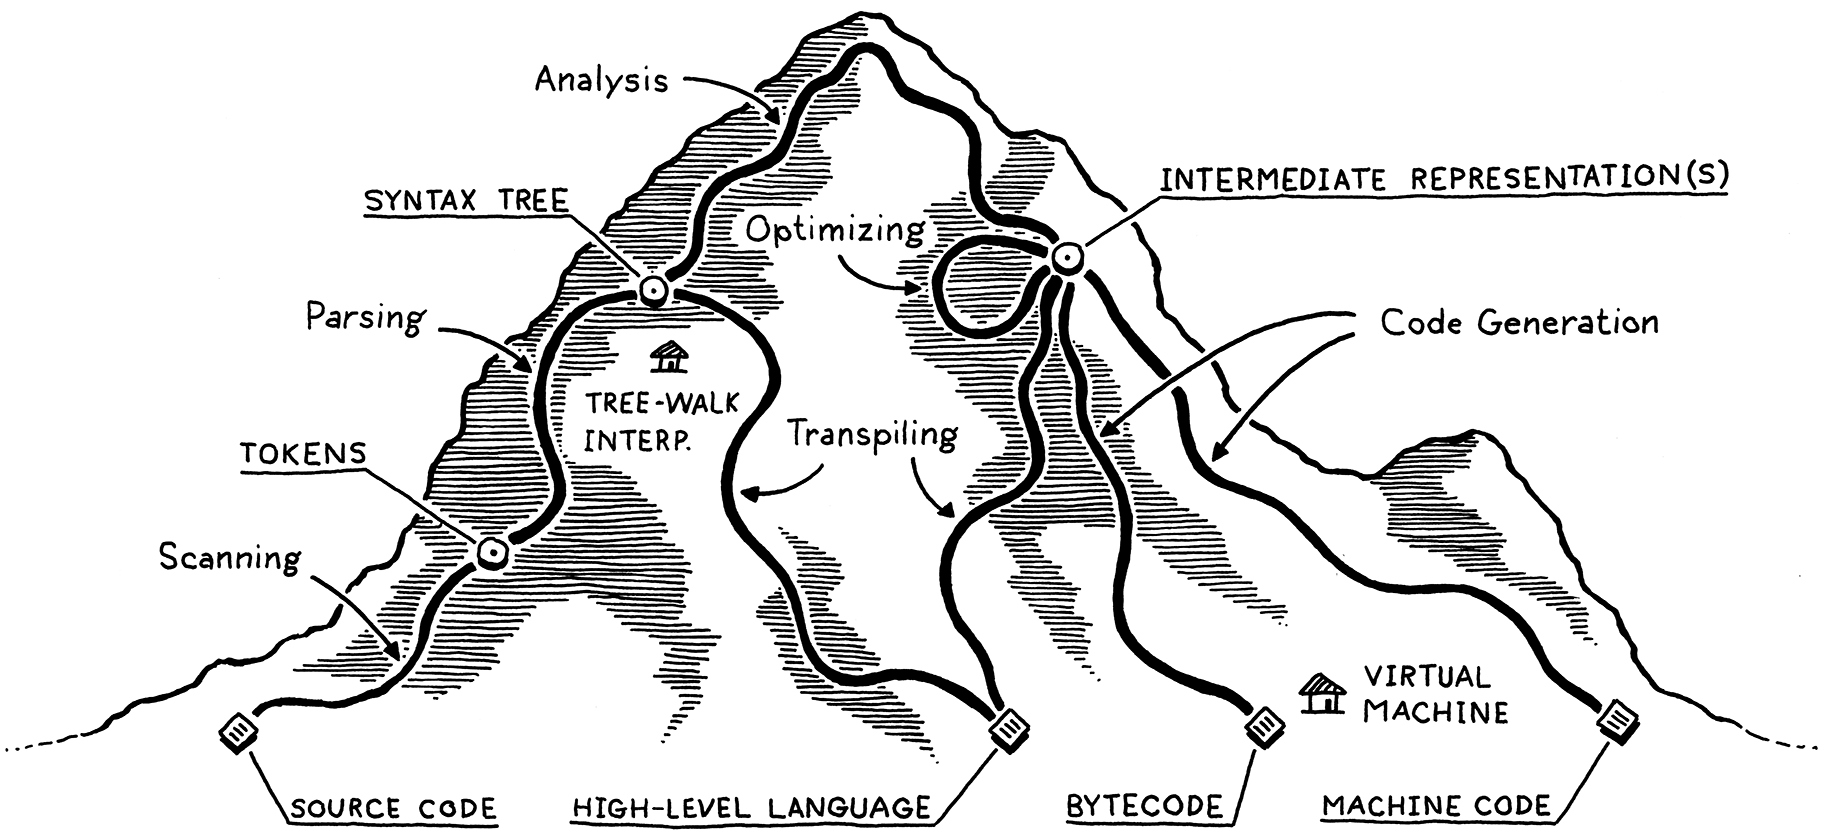
\includegraphics[scale=0.15]{resources/mountain.png}
    \caption{Schritte, die ein Compiler durchläuft \cite{Compiler:Mountain}}
    \label{fig:mountain}
\end{figure}

In diesem \textbf{TEXT} werde ich mich nur auf die im unteren Schema dargestellten Schritte fokussieren.

\begin{figure}[h!]
    \centering
    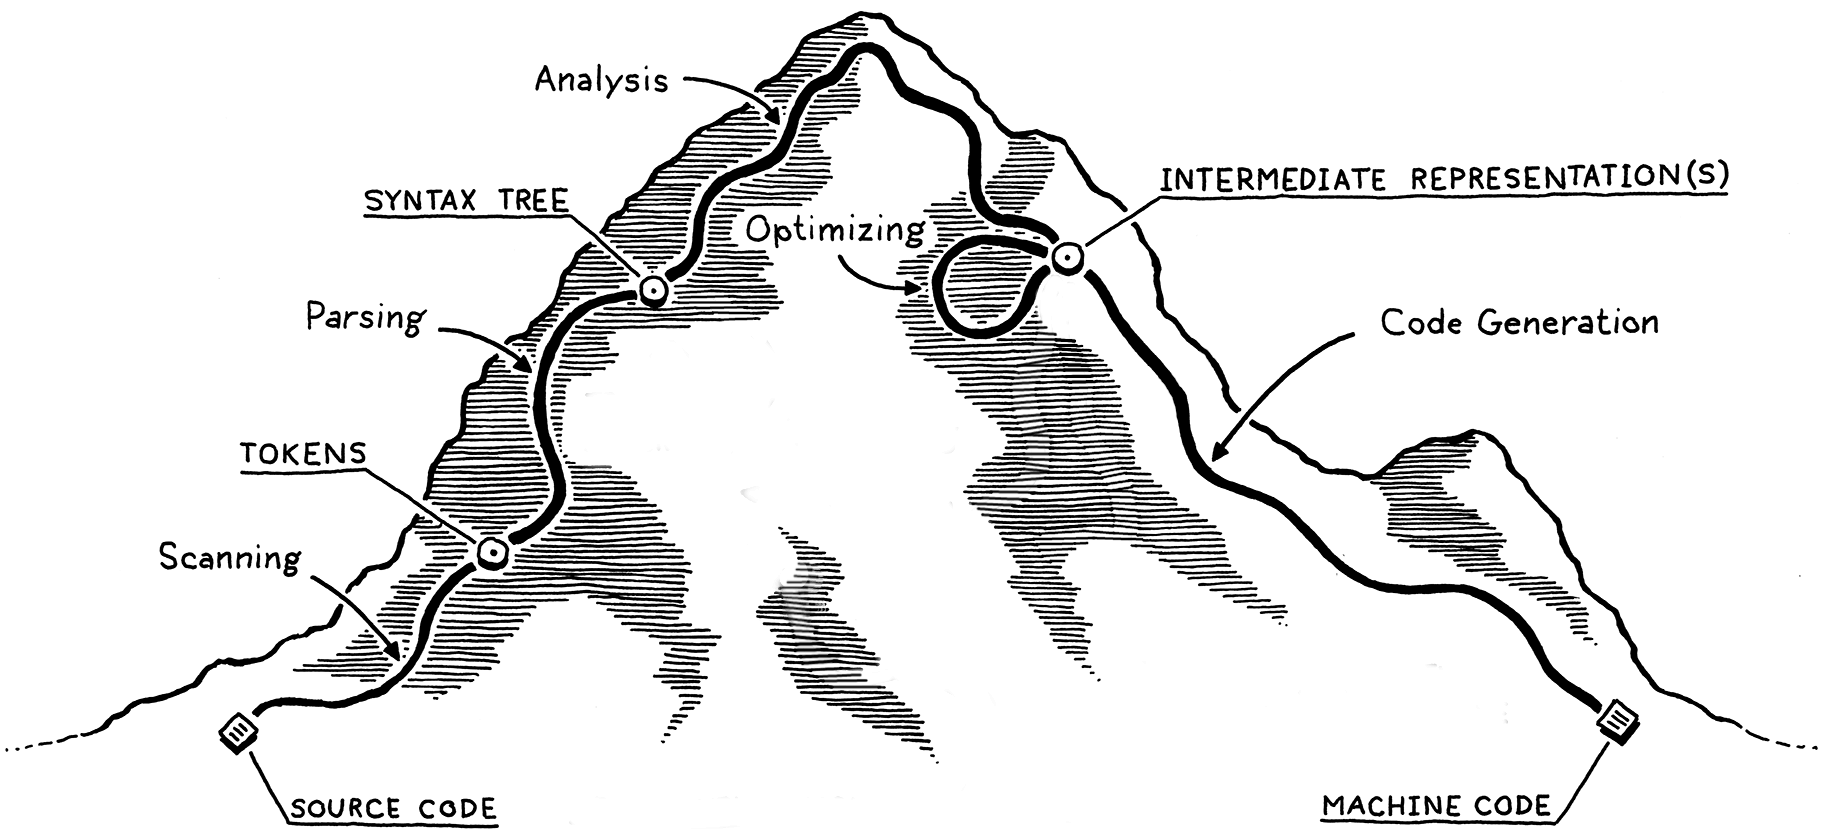
\includegraphics[scale=0.15]{resources/mountain-edited.png}
    \caption{Schritte, die in diesem \textbf{TEXT} behandelt werden (Basierend auf Figure \ref{fig:mountain})}
    \label{fig:mountain-edited}
\end{figure}

\section{Scanning}
Meist werden Programme so geschrieben, dass wir Menschen es lesen und verstehen können. Dafür verwendet man Buchstaben und Zahlen, Zeichen, wie +, *, oder Klammern, und Whitespaces, wie Leerzeichen oder Absätze.
Diese Zeichen sind jedoch für den Computer unverständlich. Der erste Schritt beim compilieren ist daher das Scannen. Dies wird von einem Teil des Compilers, dem Lexer, durchgeführt.
Die Aufgabe dieses Lexers ist es den Input File zu scannen und die gescannten Zeichen in sogenannte Tokens zu verwandeln. Diese Tokens sind Datenstrukturen, die der Compiler kennt und mit denen er weiterarbeiten kann.

Als Beispiel:

\begin{lstlisting}[language=C, label=ex:preScan, caption=C code vor dem Scannen]

int foo()
{
    if (bar == 0)
    {
        return 0;
    }

    return 1;
}

\end{lstlisting}

Würde hierbei zu einem Array von Token Objekten umgewandelt werden:

\begin{lstlisting}[label=ex:postScan, caption=Tokens nach dem Scannen]
KeywordToken (keyword="int")
IdentifierToken (id="foo")
LParenthesisToken
RParenthesisToken
KeywordToken (keyword="if")
LParenthesisToken
IdentifierToken (id="bar")
OperatorToken (operator=ComparisonEqual)
LiteralIntToken (value=0)
[...]
\end{lstlisting}

Der Lexer legt hierbei fest welche Zeichen die Input-Programmiersprache enthalten darf und welche Bedeutung ihnen Zugesprochen wird. So ist zum Beispiel im Lexer festgelegt, dass ein + Zeichen als Addition interpretiert wird.
Genauso wie im Listing \ref{ex:postScan} 'if' als KeywordToken gescannt wird, lässt sich im Lexer auch bestimmen, dass ein Wort wie 'print' als Keyword angesehen werden soll.

\section{Parsing}
Nun versteht der Compiler was mit den Zeichen im Input File gemeint ist, jedoch fehlt noch etwas bis tatsächlich in einer andere Programmiersprache übersetzt werden kann. Und das ist Verständnis für Syntax.
Die meisten High-Level Programmiersprachen weisen Syntaxregeln auf. Diese beinhalten, wie Funktionen und Variablen definiert werden oder mit welchen Punktvorstrich-Regeln Expressions evaluiert werden.
Die beim Scanning gefundenen Tokens werden nun ineinander verschachtelt und in einen sogenannten Abstract Syntax Tree (AST) überführt.

\begin{figure}[h!]
    \centering
    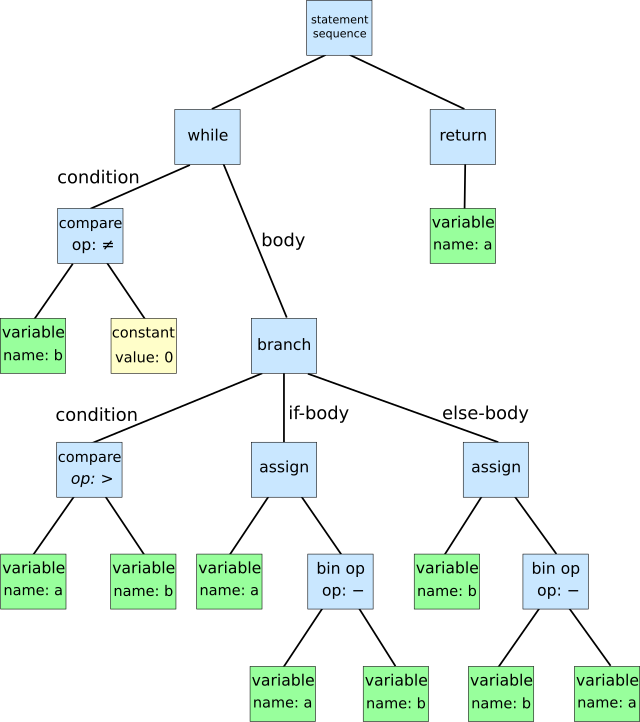
\includegraphics[scale=0.3]{resources/syntaxtree.svg.png}
    \caption{Abstract Syntax Tree zum Euklidischen Algorithmus \cite{Parser:SyntaxTree}}
    \label{fig:syntax-tree}
\end{figure}

Ein AST enthält somit nicht nur Informationen über die Tokens, sondern über die gesamte Struktur die sich aus den Tokens ergibt. Variabel- und Funktionsdefinitionen oder komplexe Statements wie 'if' oder 'for' sind hierbei im AST enthalten.
[...]

\section{Semantic Analysis}
Wie auch bei den meisten Menschensprachen gibt es auch für Programmiersprachen eine Semantik und diese muss natürlich vom Compiler verstanden werden. [...]


\section{Code Generation}
Code Generation ist der finale und oft auch komplexeste Schritt, der ein Compiler ausführen muss. Nun da unser Input-Code nicht mehr nur als Textfile, sondern als Intermediate Representation vorliegt, kann endlich Output-Code generiert werden.
Jedoch lässt sich über diesen Schritt fast am wenigsten sagen, da er je nach Output-Sprache sehr unterschiedlich aussehen kann. 

\section{Optimization}
Code Generation ist zwar der letzte Schritt beim Compilieren, trotzdem wurde eine wichtige Aufgabe des Compilers noch nicht betrachtet. Optimization ist ein Sprache die zwischen jedem der genannten Schritte geschiet.
Dabei geht es darum den Output-Code so effizient wie möglich zu machen. Effizient kann hierbei jedoch viel Verschiedenes bedeuten. Der Output-Code muss so schnell wie möglich ausgeführt werden können, Memory sparsam verwenden
und am besten auch noch ein kleiner File sein. Optimization reicht vom Entfernen der Kommentare beim Scannen oder umstellen von mathematischen Operationen bis zu entfernen von ungebrauchten Variablen und Deadstores.
Es muss von CPU Registern profitiert, mit Heap-Memory umgegangen und von inline Funktionen Gebrauch gemacht werden. Compiler Optimization ist somit ein sehr vielseitiges Problem, dass hierbei nicht weiter thematisiert werden sollte.
